\documentclass[10pt,a4paper]{article}
\usepackage[a4paper,margin=2cm]{geometry}
\usepackage[T1]{fontenc}
\usepackage[utf8]{inputenc}
\usepackage{amsmath,amssymb}
\usepackage{graphicx}
\usepackage{booktabs}
\usepackage{xcolor}
\usepackage{enumitem}
\usepackage{hyperref}
\hypersetup{colorlinks=true,urlcolor=blue!70!black,linkcolor=black}
\setlength{\parskip}{4pt}
\setlength{\parindent}{0pt}

\title{\textbf{IARA — Modelagem Preditiva e Mosaico SAR}\\
\large Space Apps 2026 · Metodologia condensada}
\author{Pipeline treinado em RTX 5090 (pod Lium) · 15.11.2026}
\date{}

\newcommand{\tune}[1]{\textcolor{orange!70!black}{\textit{#1}}}

\begin{document}
\maketitle
\vspace{-1.5em}

Documento curto descrevendo as fórmulas originais, hiperparâmetros (em
\tune{laranja}) e métricas de qualidade de cada um dos três modelos preditivos
(YANO/ENCH/SECA) e do pipeline de mosaico SAR. Hiperparâmetros marcados em
laranja foram ajustados empiricamente (tuning); os demais são padrão da
literatura ou da implementação de referência.

% ============================================================
\section{Mosaico SAR NISAR (OpenCV detail pipeline)}
% ============================================================

Cada cenário (YANO/ENCH/SECA) baixa dezenas de cenas NISAR L-band (browse PNG,
axis-aligned em \texttt{EPSG:4326}) do catálogo ASF e compõe um mosaico único.

\subsection*{Pré-processamento por cena}

Dada a imagem RGBA de uma cena $I \in \mathbb{R}^{H \times W \times 4}$:

\begin{enumerate}[leftmargin=1.2em,itemsep=0pt]
  \item \textbf{Edge-crop}: remove-se $k$ pixels de cada borda e encolhe-se o
  bbox proporcionalmente,
  $I' = I[k:H-k,\;k:W-k]$, com $k=\tune{96}$ px. Elimina a franja escura de
  queda de ganho da antena no limiar do \textit{swath}, preservando overlap
  entre passagens vizinhas.

  \item \textbf{Máscara de validade}: $M = \mathbb{1}[\alpha(I') > 0]$. Cenas
  com $\sum M < 2000$ são descartadas como ruído.
\end{enumerate}

\subsection*{Exposure compensation (global least-squares)}

Para $N$ cenas $\{I_i\}$ com sobreposições $O_{ij}$ par-a-par, estima-se um ganho
$g_i \in \mathbb{R}^3$ por canal que minimiza o resíduo de intensidade nos
pixels sobrepostos:
\begin{equation}
  \hat{g} \;=\; \arg\min_{g \in \mathbb{R}^{3N}}
  \sum_{i<j} \sum_{p \in O_{ij}} \big\| g_i \odot I_i(p) - g_j \odot I_j(p) \big\|^2.
\end{equation}
Implementação: \texttt{cv2.detail.ChannelsCompensator} (3 graus de liberdade
por cena, custo $\mathcal{O}(N)$). Testamos a variante \texttt{BlocksChannels}
($\mathcal{O}(N \cdot B^2)$) mas inviável em memória para $N\!\approx\!190$
cenas e canvas $2560\times2304$. As cenas entram no solver em versão
down-sampled ($s = \tune{0.405}$) para caber na RAM; os ganhos são aplicados em
resolução cheia.

\subsection*{Multi-band blending (pirâmide de Laplaciano)}

Cada cena é decomposta em $B$ bandas de frequência via pirâmide Laplaciana e
fundida com a máscara ponderada também em pirâmide (Burt \& Adelson, 1983):
\begin{equation}
  L_b^{\text{out}}(p) \;=\;
  \frac{\sum_i L_b(I_i)(p) \cdot G_b(M_i)(p)}{\sum_i G_b(M_i)(p)},
  \quad b=0,\dots,B-1,
\end{equation}
onde $G_b$ é o nível $b$ da pirâmide Gaussiana da máscara e $L_b$ é a diferença
de dois níveis Gaussianos consecutivos. O resultado é reconstruído somando as
pirâmides Laplacianas. Parâmetro: $B=\tune{5}$ ($2^5 = 32$ px de raio de
mistura em baixa frequência). Testamos $B=8$ e produziu \textit{halos} brilhantes
onde pixels escuros da borda contaminam faixas largas — $B=5$ é o sweet-spot.

\subsection*{Alternativa (quick-fix, no fallback \texttt{build-nisar-mosaic.py})}

Quando o pipeline OpenCV não está disponível, usamos uma normalização por
luminância escalar $L = (R+G+B)/3$ que preserva a razão HH/HV do falso-colorido
DHDH:
\begin{align}
  s &= \frac{T_{hi} - T_{lo}}{\max(p_{98}(L_i) - p_{2}(L_i), \varepsilon)}, \qquad
  o = T_{lo} - s \cdot p_{2}(L_i), \\
  I_i' &= \text{clip}(s \cdot I_i + o,\; 0,\; 255).
\end{align}
onde $(T_{lo}, T_{hi})$ é a mediana dos percentis $(\tune{p_2}, \tune{p_{98}})$
sobre todas as cenas. Depois aplica-se feathering gaussiano no canal alpha com
$\sigma=\tune{4}$ px e composição por $\alpha$-blend.

% ============================================================
\section{YANO — Risco de garimpo (XGBoost)}
% ============================================================

\textbf{Alvo}: probabilidade de um pixel $250\,\text{m} \times 250\,\text{m}$
sofrer perda florestal (proxy para expansão de garimpo) no próximo ano, usando
Hansen GFC v1.12 como rótulo.

\subsection*{Features (11 por pixel)}

$(x, y)$ em UTM, distância ao garimpo existente DETER, distância ao rio,
elevação SRTM, slope SRTM, Sentinel-1 RTC $\sigma^0$ em VV e VH (mediana
anual), Hansen \textit{cumulative loss} em buffer 1~km até $t$, distância ao
pixel de perda mais próximo, chuva CHIRPS somada no ano, e \texttt{year\_norm}
$=(y-2020)/5$.

\subsection*{Modelo}

Gradient-boosted trees (\texttt{xgboost} GPU \texttt{tree\_method=hist}). A
previsão é o produto sigmoid das somas das folhas:
\begin{equation}
  \hat{p}(x) = \sigma\!\left(\sum_{m=1}^{M} f_m(x)\right),
  \qquad f_m \in \mathcal{F}_{\text{trees}}.
\end{equation}
Minimiza o \textit{binary logistic loss} com regularização quadrática
$\lambda \|\mathbf{w}\|^2$:
\begin{equation}
  \mathcal{L} = \sum_i \ell(y_i, \hat{p}_i) + \sum_m \Omega(f_m),
  \quad \Omega(f) = \gamma T + \tfrac{1}{2}\lambda \|w\|^2.
\end{equation}

Hiperparâmetros: \tune{$M=800$}, \tune{$d_{\max}=6$}, \tune{$\eta=0.05$},
\tune{subsample $=0.8$}, \tune{colsample\_bytree $=0.8$}, $\lambda=1$,
\texttt{scale\_pos\_weight} $= n_{\text{neg}}/n_{\text{pos}}$, \tune{early
stopping em 50 rodadas} (métrica interna \texttt{aucpr}).
Split temporal: treino 2019–2022, teste 2023.

\subsection*{Qualidade (holdout 2023)}

\begin{center}
\small
\begin{tabular}{lrrrrr}
\toprule
Split & $n$ & $n^+$ & ROC-AUC & PR-AUC & recall@top-5\% \\
\midrule
train (2019–2022) & 472\,500 & 4\,339 & 0.931 & 0.317 & 0.796 \\
test (2023) & 157\,500 & 1\,706 & 0.797 & 0.157 & 0.518 \\
\bottomrule
\end{tabular}
\end{center}

Brier test $= 0.080$. Interpretação: entre os 5\% de pixels mais arriscados
previstos, capturamos \textbf{51{,}8\%} de todos os pixels que efetivamente
sofreram perda em 2023.

\begin{center}
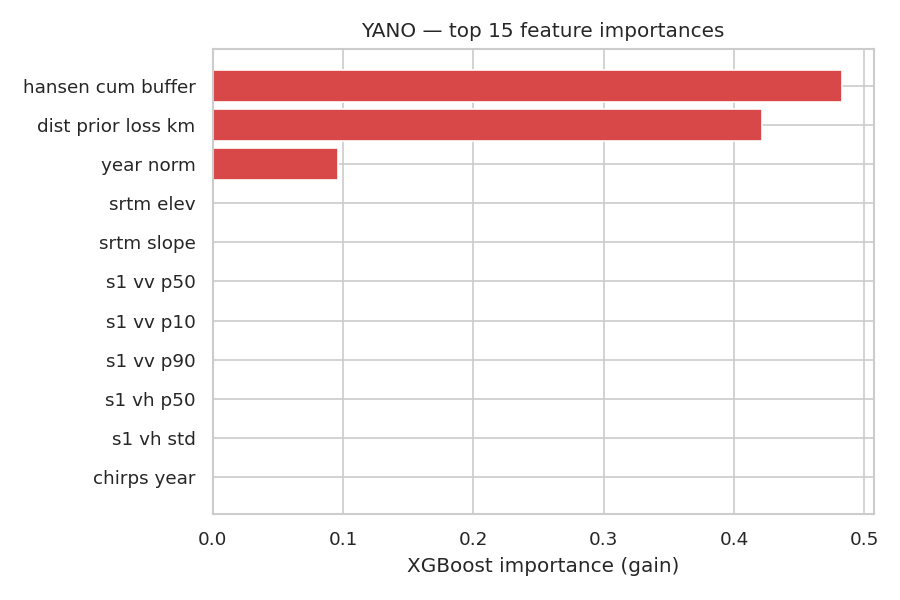
\includegraphics[width=0.82\linewidth]{../outputs/fig_yano_feature_importance.png}
\end{center}
\textit{Importância das features (gain). A distância a perda anterior
(\texttt{dist\_prior\_loss\_km}) é o sinal mais forte — garimpo avança a partir
de frentes já abertas.}

% ============================================================
\section{ENCH — Cota do Rio Negro (SARIMAX + LSTM)}
% ============================================================

\textbf{Alvo}: nível diário do Rio Negro na régua ANA 14990000 (Porto de
Manaus), com horizontes $h \in \{7,\,30,\,365\}$ dias. Dados: 1902–2014 (API
ANA SOAP legacy limitada a essa janela).

\subsection*{Features exógenas}

Termos de Fourier anuais $m=365{.}25$:
\begin{equation}
  \phi_k(t) = \left(\sin\!\tfrac{2\pi k t}{m},\;\cos\!\tfrac{2\pi k t}{m}\right),
  \quad k=1,\dots,K,\;\; K=\tune{3}.
\end{equation}
Mais ENSO com \tune{lag de 180 dias} (Niño 3.4 $z$-score mensal, SOI):
$\mathbf{x}_t = [\text{nino34}_{t-180},\;\text{soi}_{t-180},\;\phi_1,\dots,\phi_3]$.

\subsection*{Baseline — SARIMAX$(p,d,q)(P,D,Q)_s$}

\begin{equation}
  \Phi_P(B^s)\phi_p(B)(1-B)^d(1-B^s)^D y_t
  = \Theta_Q(B^s)\theta_q(B)\,\epsilon_t + \boldsymbol{\beta}^\top \mathbf{x}_t.
\end{equation}
Configuração: $(p,d,q)=\tune{(1,1,0)}$, $(P,D,Q,s)=(0,0,0,0)$ (sazonalidade
absorvida pelos Fourier). Ajuste L-BFGS, 50 iterações máx. Previsão do
holdout 2010--2014 com banda de confiança 80\% direto do estado filtrado.

\subsection*{Challenger — LSTM}

Janela de 365 dias passados concatenada com exógenas, prevê $y_{t+h}$:
\begin{align}
  h_t, c_t &= \text{LSTM}(\mathbf{u}_t, h_{t-1}, c_{t-1}), \\
  \hat{y}_{t+h} &= W_o h_t + b_o.
\end{align}
Arquitetura: $2$ camadas de \tune{hidden $=128$}, dropout $=0{.}1$, cabeça
linear. Treino: Adam$W$ (\tune{lr $=10^{-3}$}), Huber loss, \tune{30 epochs},
batch 512. Normalização $z$-score ajustada apenas no train split.

\subsection*{Qualidade (holdout 2010–2014, $n$=1825 dias)}

\begin{center}
\small
\begin{tabular}{lrrrr}
\toprule
Modelo & RMSE (m) & MAE (m) & NSE & peak-RMSE P90 (m) \\
\midrule
SARIMAX (1-step) & 1.820 & 1.522 & 0.815 & 2.050 \\
LSTM $h=7$~d & \textbf{0.200} & \textbf{0.138} & \textbf{0.998} & \textbf{0.117} \\
LSTM $h=30$~d & 0.958 & 0.716 & 0.949 & 0.304 \\
LSTM $h=365$~d & 2.184 & 1.828 & 0.707 & 1.816 \\
\bottomrule
\end{tabular}
\end{center}

NSE (Nash–Sutcliffe) $=1$ seria predição perfeita; $>0{.}7$ é considerado
``bom'' em hidrologia operacional. Peak-RMSE P90 é o RMSE restrito aos dias
cuja observação está acima do percentil 90 — mede erro no \textit{pico} da cheia,
que é onde a decisão humana importa.

\begin{center}
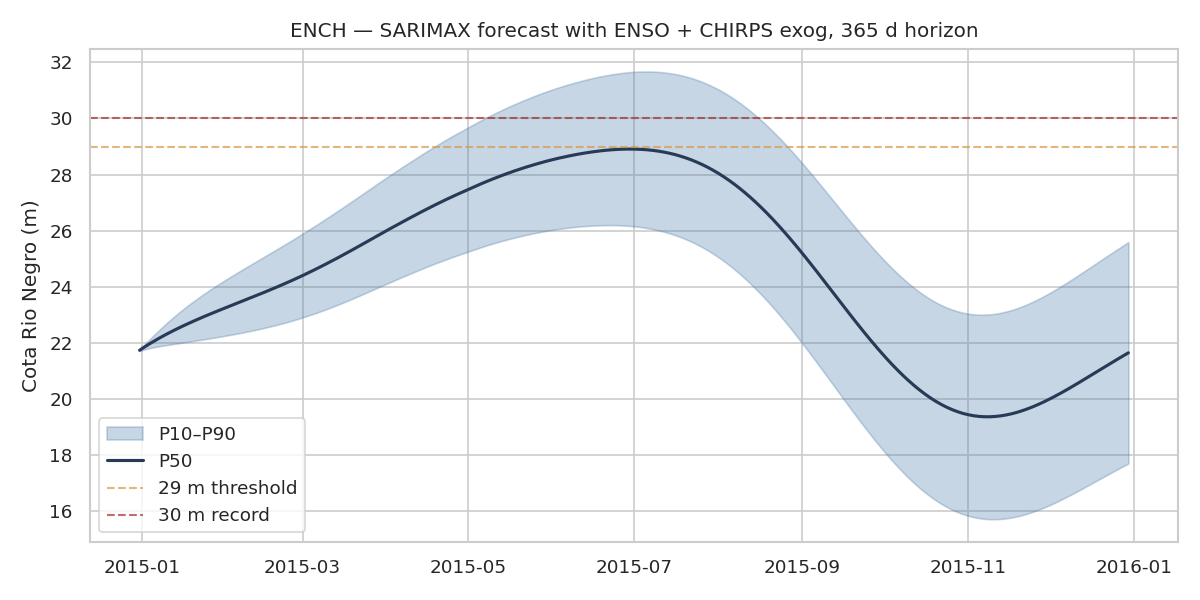
\includegraphics[width=0.90\linewidth]{../outputs/fig_ench_forecast.png}
\end{center}
\textit{Previsão SARIMAX com banda P10–P90 vs observado 2010–2014. Linhas
tracejadas marcam as cotas oficiais SGB: 27{,}50 m atenção, 29{,}00 m inundação,
29{,}97 m inundação severa.}

% ============================================================
\section{SECA — Isolamento de comunidades (Logístico + Monte Carlo)}
% ============================================================

\textbf{Alvo}: probabilidade diária de uma comunidade ribeirinha
$c \in \{\text{Andiroba, Jutaí, Barro Alto, Janauacá}\}$ ficar isolada,
condicionada ao nível do Rio Negro.

\subsection*{Rótulo persistente}

Um único dia abaixo do limiar $\tau_c$ não configura isolamento. Usamos:
\begin{equation}
  y_{c,t} = \mathbb{1}\!\left[\sum_{k=0}^{6} \mathbb{1}[y_{t-k} < \tau_c]\ \ge\ 7\right],
\end{equation}
isto é, janela deslizante de \tune{7 dias consecutivos} abaixo do limiar. O
limiar $\tau_c$ é o quantil histórico calibrado por comunidade — Andiroba
$\tau=19{.}86$~m, Jutaí $\tau=18{.}36$, Barro Alto $\tau=17{.}38$, Janauacá
$\tau=16{.}36$. Fonte dos limiares: cadastro IBGE 2022 + registros de acesso
das comunidades (lago/paraná).

\subsection*{Classificador logístico}

\begin{equation}
  \text{logit}\,P(y_{c,t}=1 \mid \mathbf{z}_t) = \beta_0 + \beta_1 (y_t - \tau_c)
  + \beta_2 \sin\!\tfrac{2\pi m_t}{12} + \beta_3 \cos\!\tfrac{2\pi m_t}{12}.
\end{equation}
\texttt{sklearn.LogisticRegression} com \tune{$C=1$}, \texttt{max\_iter}$=1000$,
\tune{class\_weight = balanced}. Split 80/20 temporal.

\subsection*{Monte Carlo sobre a previsão do Rio Negro}

A banda $(p_{10}, p_{50}, p_{90})_t$ do forecast ENCH é tratada como Gaussiana
$\mathcal{N}(\mu_t, \sigma_t^2)$ com
\begin{equation}
  \sigma_t = \frac{p_{90,t} - p_{10,t}}{2\,\Phi^{-1}(0{.}9)}, \qquad \mu_t = p_{50,t}.
\end{equation}
Simulamos $n=\tune{2000}$ trajetórias $\{\tilde{y}_t^{(k)}\}$. Para cada
trajetória, aplicamos o classificador logístico → vetor diário
$\{\hat{p}_{c,t}^{(k)}\}$ e extraímos a soma anual $D_c^{(k)} = \sum_t \tilde{y}_{c,t}^{(k)}$
(dias isolados no horizonte de 365 dias). Resultados reportados: $(p_{10},
p_{50}, p_{90}, \text{mean})$ de $\{D_c^{(k)}\}_{k=1}^{n}$.

\subsection*{Qualidade (holdout 2010–2014)}

\begin{center}
\small
\begin{tabular}{lrrrr}
\toprule
Comunidade & $n_{\text{test}}$ & $n^+$ & ROC-AUC & Brier \\
\midrule
Andiroba    & 8\,203 & 1\,468 & 0.999 & 0.0108 \\
Jutaí       & 8\,203 & 771    & 0.999 & 0.0098 \\
Barro Alto  & 8\,203 & 433    & 0.999 & 0.0095 \\
Janauacá    & 8\,203 & 214    & 1.000 & 0.0064 \\
\bottomrule
\end{tabular}
\end{center}

ROC-AUC quase perfeito reflete o fato de que o rótulo persistente é quase
determinístico dado o nível observado --- o valor agregado está na propagação
Monte Carlo da \emph{incerteza do forecast} ENCH, que transforma uma
probabilidade por dia em uma distribuição de dias isolados.

% ============================================================
\section*{Apêndice: hiperparâmetros com tuning}
% ============================================================

\begin{center}
\small
\begin{tabular}{lll}
\toprule
Símbolo & Componente & Valor escolhido \\
\midrule
$k$ (edge-crop px) & Mosaico NISAR & 96 (teste: 24, 48, 96, 128) \\
$s$ (feed scale) & Exposure compensation & 0.405 \\
$B$ (num bands) & Multi-band blender & 5 (teste: 5, 8) \\
$\sigma$ (alpha feather) & Fallback quick-fix & 4 px \\
$(p_2, p_{98})$ & Normalização percentil & (2, 98) \\
$M$ (n\_estimators) & YANO XGBoost & 800 \\
$d_{\max}$ & YANO XGBoost & 6 \\
$\eta$ (learning rate) & YANO XGBoost & 0.05 \\
subsample, colsample & YANO XGBoost & 0.8, 0.8 \\
early stopping & YANO XGBoost & 50 rodadas \\
$(p,d,q)$ & ENCH SARIMAX & (1, 1, 0) \\
$K$ Fourier & ENCH exógenas & 3 \\
lag ENSO & ENCH exógenas & 180 dias \\
hidden size & ENCH LSTM & 128 \\
layers, dropout & ENCH LSTM & 2, 0.1 \\
epochs, lr & ENCH LSTM & 30, $10^{-3}$ \\
batch size & ENCH LSTM & 512 \\
janela de persistência & SECA rótulo & 7 dias \\
$C$, class\_weight & SECA logístico & 1.0, balanced \\
$n$ Monte Carlo & SECA simulação & 2000 \\
\bottomrule
\end{tabular}
\end{center}

\vspace{0.5em}
\footnotesize
\textbf{Dados fonte:} Hansen GFC v1.12 (Landsat/NASA); Sentinel-1 RTC
(Microsoft Planetary Computer); SRTM GL1 30~m; ANA 14990000 (1902–2014);
NOAA ERSST Niño 3.4 + SOI; DETER-Amz MINERACAO (INPE TerraBrasilis); CHIRPS
daily v2.0; JRC Global Surface Water Yearly 2024; Hutukara e SESAI DSEI-Y
(coordenadas de polo-base Yanomami).

\end{document}
